%
% main.tex -- Paper zum Thema <buchberger>
%
% (c) 2026 Nathanael Fässler, OST Ostschweizer Fachhochschule
%
% !TEX root = ../../buch.tex
% !TEX encoding = UTF-8
%
\chapter{Lösung von Polynomgleichungen\label{chapter:buchberger}}
\kopflinks{Lösung von Polynomgleichungen}
\begin{refsection}
\chapterauthor{Nathanael Fässler}

An der OST lernen Studenten der technischen Studiengänge in Vorlesungen der linearen Algebra, wie man lineare Gleichungssysteme löst.
Dafür lernen sie den Gauss-Algorithmus kennen.
Mit diesem Verfahren lässt sich allerdings nur eine Teilmenge von Problemen mit Gleichungssystemen lösen.
Um Gleichungssysteme mit Polynomgleichungen zu lösen, braucht man ein mächtigeres Werkzeug: den Buchberger-Algorithmus.

Dieses Paper erklärt die Erweiterung von linearen Gleichungssystemen zu polynomiellen Gleichungssystemen und wie man sie löst.
Im Kapitel~\ref{buchberger:section:sudoku} wird als interessante Anwendung ein Sudoku in ein Gleichungssystem aus Polynomgleichungen übersetzt und anschliessend mit dem Buchberger-Algorithmus gelöst.

%
% einleitung.tex
%
% (c) 2026 Nathanael Fässler, OST Ostschweizer Fachhochschule
%
% !TEX root = ../../buch.tex
% !TEX encoding = UTF-8
%
\section{Lineare Gleichungssysteme
\label{buchberger:section:teil0}}
\kopfrechts{Lineare Gleichungssysteme}
Viele Elemente des Gauss-Algorithmus werden in einer ähnlichen Form wiederkehren, im Kapitel zum Buchberger-Algorithmus~\ref{buchberger:section:buchberger}. 
Daher ist es empfehlenswert die Grundideen des Lösens eines linearen Gleichungssystems zu repetieren.

Das Gleichungssystem
\begin{equation}
  \begin{cases}
  x + 2y = 3 \\
  3x - y = 15
  \end{cases}
\label{buchberger:lineares-gleichungssystem-1}
\end{equation}
lässt sich bekanntlicherweise mit dem Gauss-Algorithmus lösen.
Das Vorgehen ist wie folgt:
\begin{enumerate}
\item
Die Gleichungen werden in eine passende Form gebracht:

Alle Terme mit einer Variable werden auf die linke Seite gebracht während auf der rechten Seite der konstante Wert steht.
Die Reihenfolge der Variablen muss einer festgelegten Ordnung folgen damit der Algorithmus deterministisch ist.
Das Gleichungssystem~\eqref{buchberger:lineares-gleichungssystem-1} ist bereits in dieser Form, wobei die Ordnung dadurch gegeben ist, dass $x$ vor $y$ steht.
\item
Mit iterativen Gleichungsumformungen, die hier nicht weiter relevant sind, wird das Gleichungssystem in eine treppenartige Form gebracht.
\begin{equation}
  \begin{cases}
  x + 2y = 3 \\
  0x + y = -\frac{6}{7}
  \end{cases}
  \label{buchberger:lineares-gleichungssystem-2}
\end{equation}
\item
Aus dem Gleichungssystem~\eqref{buchberger:lineares-gleichungssystem-2} lässt sich direkt die Lösung für $y$ ablesen, welche $-\frac{6}{7}$ beträgt.
Diese Lösung für $y$ lässt sich in der oberen Gleichung einsetzen.
Dabei wird eine Gleichung erreicht die nur noch $x$ enthält. Das Auflösen nach $x$ ist trivial.
\end{enumerate}

Der Algorithmus lässt sich auf beliebig grosse Gleichungssysteme anwenden:

Bei einem Gleichungssystem mit den Variablen $x_{0}, x_{1}, \dots, x_{n}$ erhält man nach dem anwenden des Gauss-Algorithmus eine Zeilenstufenform,
wobei in der untersten Gleichung nur noch die Variable $x_{n}$ vorkommt und deren Lösung sich direkt ablesen lässt.
Die nächsthöhere Gleichung lässt sich dann iterativ lösen indem man immer die Lösungen der bereits fixierten Variablen einsetzt.

Bemerkenswert ist, dass ein zunächst schwer lösbares Gleichungssystem in ein äquivalentes\footnote{Zwei Gleichungssysteme sind äquivalent, wenn sie exakt dieselbe Lösungsmenge besitzen.} Gleichungssystem umgewandelt wird, welches einfacher lösbar ist.
%
% buchberger.tex
%
% (c) 2026 Nathanael Fässler, OST Ostschweizer Fachhochschule
%
% !TEX root = ../../buch.tex
% !TEX encoding = UTF-8
%
\section{Polynomielle Gleichungssysteme
\label{buchberger:section:buchberger}}
\kopfrechts{Polynomielle Gleichungssysteme}
Das Gleichungssystem
\begin{equation}
  \begin{cases}
  x^2 -y = 0 \\
  x + y^2 = 3
  \end{cases}
  \label{buchberger:polynom-gleichungssystem-1}
\end{equation}
lässt sich nicht mehr mit dem Gauss-Algorithmus lösen.
Der Grund ist, dass es Variablen mit Potenzen $> 1$ beinhaltet, also nicht linear.

Um solche nonlineare multivariate\footnote{Multivariat bedeutet, dass mehrere Variablen vorkommen.} Gleichungssysteme zu lösen eignet sich der Buchberger-Algorithmus.
Ein Gleichungssystem wie
\begin{equation}
  \begin{cases}
  5xy + 2y^3 +  5y^8z + z^3 = 100 \\
  3x^2y^4z^9 + 2z^2 = 1 \\
  (x-1)\,(y-2)\,(z-3) = 0 \\
  \end{cases}
  \label{buchberger:polynom-gleichungssystem-2}
\end{equation}
lässt sich damit auch lösen.

Terme mit mehreren Variablen wie $5xy$ sind hier im Gegensatz zu linearen Gleichungen erlaubt.
Die Klammern der letzten Gleichung stellen kein neues Problem dar, da sie beim ausmultiplizieren auch in die bekannte Koeffizientenform gebracht werden können.


\subsection{Geschichte}
\label{buchberger:subsection:geschichte}
Im Jahre 1965 hat der österreichische Mathematik-Student Bruno Buchberger in seiner Dissertation die Gröbner-Basis entwickelt.
Er hat sie nach seinem Professor Wolfgang Gröbner benannt.
Zu seiner Dissertation gehörte auch der Buchberger-Algorithmus mit dem man Gröbner-Basen berechnen kann.
Der Algorithmus wurde zu einem wichtigen Bestandteil von Computeralgebrasystemen.

\subsection{Buchberger-Algorithmus}
\label{buchberger:subsection:buchberger-algorithmus}

\begin{algorithm}
\caption{Pseudo-Code des Buchberger-Algorithmus in C++/Java ähnlichem Style
\label{buchberger:pseudo-code}}
\begin{algorithmic}[1]
  \State \textbf{function} Buchberger(Menge$<$Polynom$>$ startPolynome) \{
    \State \quad Menge$<$Polynom$>$ basis = startPolynome;
    \State \quad Menge$<$Polynom$>$ alteBasis = \{\};
    \State \quad \textbf{while} (basis $\neq$ alteBasis) \{
      \State \quad \quad alteBasis = basis;
      \State \quad \quad \textbf{for} (Pair$<$Polynom$>$ (p, q) $\in$ alteBasis) \{
        \State \quad \quad \quad Polynom rest = spezialDivision((p, q), alteBasis);
        \State \quad \quad \quad \textbf{if} (rest $\neq$ 0) \{
          \State \quad \quad \quad \quad basis = basis $\cup$ \{rest\}; \Comment{Fügt neues Polynom zur Basis hinzu.}
        \State \quad \quad \quad \} % end if
      \State \quad \quad \} % end for
    \State \quad \} % end while
    \State \quad \textbf{return} basis;
  \State \} % end function
\end{algorithmic}
\end{algorithm}

Dieses Kapitel soll dem Leser eine Idee geben wie der Buchberger-Algorithmus funktioniert und wie man ihn anwendet.
Wie der Algorithmus genau funktioniert erklärt Lamagna in seinem Buch~\cite{buchberger:computer-algebra} in Kapitel 8.%cite{buchberger:computer-algebra}

Wie beim Gauss-Algorithmus müssen die Gleichungen zunächst in eine geeignete Form gebracht werden.
Die Gleichungen werden in Polynome umgewandelt, wobei sie vorher auf die Form $p(x) = 0$ umgestellt werden.
Das Gleichungssystem
\begin{equation}
  \begin{cases}
  x^2 -y = 0 \\
  x + y^2 -3 = 0
  \end{cases}
  \label{buchberger:polynom-gleichungssystem-3}
\end{equation}
wird in die Menge der Polynome 
\begin{equation}
  B
  =
  \{
    x^2 -y,
    x + y^2 - 3
  \}
  \label{buchberger:polynom-gleichungssystem-4}
\end{equation}
umgeformt.

Dabei ist wichtig, dass alle Polynome eine eindeutige Ordnung der Terme besitzen.
Zum Beispiel legt die lexikographische Ordnung fest, dass zuerst alle Terme mit dem höchsten Grad bezüglich $x$ stehen.
Wenn dies auf mehrere Terme zutrifft, wird innerhalb dieser Gruppe bezüglich des Grads von $y$ sortiert und dann bezüglich $z$ und so weiter bis zur letzen Variable.
Dies ist nötig, da der Buchberger-Algorithmus eine spezielle Variante der Polynomdivision verwendet, wobei der leitende Term bekannt sein muss.

Der Pseudo-Code des Algorithmus~\ref{buchberger:pseudo-code} zeigt vereinfacht den Ablauf auf.
Die Funktion spezialDivision ist in sich selbst ein komplizierter Algorithmus und wird im folgenden nur grob erklärt.
s
Der Algorithmus startet mit einer Menge von Polynomen, welche die Basis genannt wird (Zeile 2).
Aus den Polynomen der Basis werden alle möglichen Paare gebildet (Zeile 4).
Mit einer speziellen Polynomdivision\footnote{Im Pseudo-Code wird die Funktion spezialDivision genannt.}(Zeile 7), die jeweils eines der Paare als Dividend und die ganze Basis als Divisor einbezieht, wird ein Quotient mit Rest berechnet.
Dabei will der Algorithmus herausfinden ob jeweils zwei Polynome als Paar eine Information tragen, die in der Basis noch nicht enthalten ist.
Darum ist auch in einer dieser Polynomdivision-Operationen immer ein Paar und die ganze Basis beteiligt.

Die neue Information die bei dieser Polynomdivision gewonnen wurde ist der Rest der Division.
Dieser Rest wird als Polynom zur Basis hinzugefügt um somit die neu gewonnene Information zu behalten (Zeile 9).
Durch die Vergrösserung der Basis haben sich auch neue Polynom-Paare ergeben.
Diese neuen Paare werden auch den Polynomdivisions-Schritt durchlaufen.

Wenn ein Paar keine neuen Informationen liefert, zeigt sich das daran, dass das Paar durch die Basis teilbar ist ohne Rest.
Also wenn der Rest $0$ ist, war das Paar nutzlos (Zeile 8).
Die Tatsache, dass das Polynom $0$ keine Information liefert macht durchaus Sinn:
Wenn man das Polynom $0$ als Gleichung interpretiert muss man es gleich Null setzen und die Gleichung $0 = 0$ ist immer wahr, und liefert keine Information.

Die Prozedur wird solange wiederholt bis keine neuen Polynome zur Basis hinzugefügt werden können (Zeile 4).
Das Resultat ist eine Basis mit mindestens so vielen Polynome wie die ursprüngliche Basis (Zeile 13).
Der Grund ist, dass nur Polynome hinzugefügt aber nie entfernt wurden.

Im letzten Schritt, der hier nicht genauer erklärt wird, und auch nicht im Pseudo-Code~\ref{buchberger:pseudo-code} enthalten ist, werden redundante Polynome entfernt und das Ergebnis ist eine sogenannte \emph{Gröbner-Basis}.

Wenn man den Algorithmus auf das System \eqref{buchberger:polynom-gleichungssystem-1} 
anwendet erhält man die Gröbner-Basis 
\begin{equation}
  G
  =
  \{
    x^4 + x - 3,
    x^2 - y
  \}
  \label{buchberger:polynom-gleichungssystem-5}
\end{equation} 
, woraus sich das Gleichungssystem
\begin{equation}
  \begin{cases}
  x^4 + x = 3 \\
  x^2 - y = 0
  \end{cases}
  \label{buchberger:polynom-gleichungssystem-6}
\end{equation}
konstruieren lässt.

Das Gleichungssystem ist zwar noch nicht gelöst, aber es besitzt eine nützliche Eigenschaft.
Nämlich, dass die erste Gleichung nur noch die Variable $x$ beinhaltet.
Eine Gleichung mit nur einer Variable lässt sich numerisch lösen mit z.B. dem \emph{Newton-Verfahren}.
Wie beim Gauss-Algorithmus erhält man beim Buchberger-Algorithmus eine Zeilenstufenform, 
wobei sich immer das Ergebnis der vorherigen Gleichungen in die nächste einsetzen lassen.
Weil es sich hier um nonlineare Gleichungen handelt, kann eine Gleichung mehrere Lösungen für eine Variable ergeben.
Beim Rückwärtseinsetzen müssen dann alle Kombinationen der bisherigen Lösungen eingesetzt werden.



\subsection{Visualisierung eines Gleichungssystems}
\label{buchberger:subsection:visualisierung}
\begin{figure}
\centering
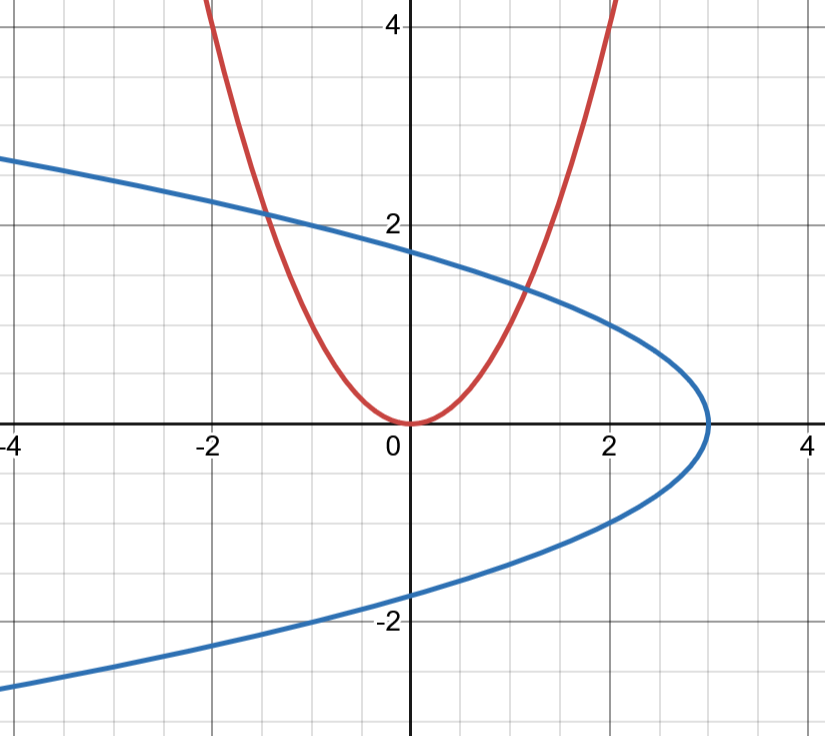
\includegraphics[width=0.7\textwidth]{papers/buchberger/images/equationSystem1.png}
\caption{Visualisierung des Gleichungssystems \protect\eqref{buchberger:polynom-gleichungssystem-1}
  \textcolor{red}{Rot: $x^2 - y = 0$},
  \textcolor{blue}{Blau: $x + y^2 = 3$}
  \label{buchberger:equationVisual1}}
\end{figure}

Der Plot~\ref{buchberger:equationVisual1}
visualisiert das Gleichungssystem \eqref{buchberger:polynom-gleichungssystem-1}
.
Alle Kombinationen von $x$ und $y$ die dazuführen, dass eine Gleichung wahr wird, sind ein Punkt auf dem roten bzw. blauen Graphen.
Die Schnittpunkte der Graphen ergeben gerade die Lösungen des Gleichungssystem.

\begin{figure}
\centering
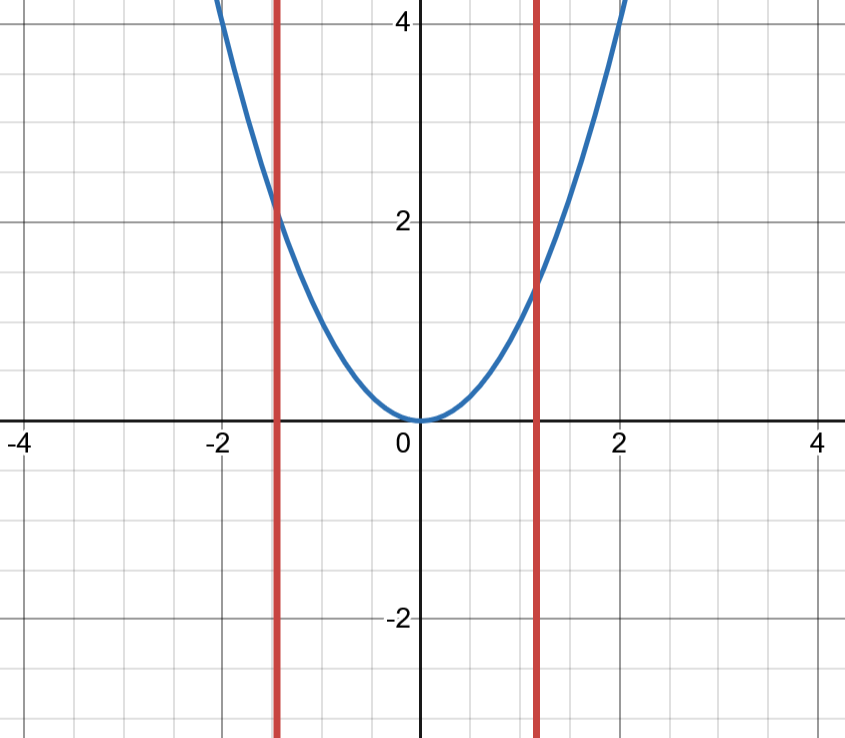
\includegraphics[width=0.7\textwidth]{papers/buchberger/images/equationSystem2.png}
\caption{Visualisierung des Gleichungssystems \protect\eqref{buchberger:polynom-gleichungssystem-6}
  \textcolor{red}{Rot: $x^4 + x = 3$},
  \textcolor{blue}{Blau: $x^2 - y = 0$}
\label{buchberger:equationVisual2}}
\end{figure}
Auf dem Plot~\ref{buchberger:equationVisual2}
ist das Gleichungssystem der Gröbner-Basis \eqref{buchberger:polynom-gleichungssystem-6}
dargestellt.
Die Eigenschaft, dass die erste Gleichung nur die Variable $x$ beinhaltet wird hier auf interessante Weise sichtbar:
Die Gleichung besteht nur noch aus vertikalen Geraden.
Das erklärt sich dadurch, dass die Gleichung nicht mehr von $y$ abhängt und somit die y-Achse nicht mehr relevant ist für die Gleichung.
Die Gleichung wurde sozusagen auf eine Dimension reduziert.
%
% sudoku.tex
%
% (c) 2026 Nathanael Fässler, OST Ostschweizer Fachhochschule
%
% !TEX root = ../../buch.tex
% !TEX encoding = UTF-8
%

% Hilfsfunktion um Sudokus zu zeichnen
\newcounter{sudokuRow}
\newcounter{sudokuCol}

\newcommand\setrow[4]{
  \setcounter{sudokuCol}{1}
  \foreach \n in {#1, #2, #3, #4} {
    \edef\x{\value{sudokuCol} - 0.5}
    \edef\y{4.5 - \value{sudokuRow}}
    \node[anchor=center, font=\Huge] at (\x, \y) {\n};
    \stepcounter{sudokuCol}
  }
  \stepcounter{sudokuRow}
}

\section{Sudoku
\label{buchberger:section:sudoku}}
\kopfrechts{Sudoku}

\begin{figure}
\centering
\input{papers/buchberger/images/sudokuUnsolved.tex}
\caption{Ein ungelöstes Sudoku.
\label{buchberger:sudokuUnsolved}}
\end{figure}
Ein Sudoku ist ein bekanntes Ausfüllrätsel, bei dem in jedes leere Feld eine Ziffer eingetragen werden muss.
Das Sudoku gilt als gelöst wenn bestimmte Regeln erfüllt sind.

Das abgebildete 4x4 Sudoku\footnote{Ein 4x4 Sudoku wird auch Shidoku genannt.} ist eine kleinere Form des üblichen 9x9 Sudokus.
Die Regeln sind gleich, aber auf die kleinere Form angepasst.
Die Struktur und Regeln eines Sudokus lassen sich mathematisch mit Gleichungen einfach modellieren.
Deshalb bietet es sich an, die Anwendung des Buchberger-Algorithmus anhand eines Sudokus zu demonstrieren.

\subsection{Variablen des Sudokus
\label{buchberger:subsection:variablen-des-sudokus}}
\begin{figure}
\centering
\input{papers/buchberger/images/sudokuVariables.tex}
\caption{Sudoku mit Variablen für alle 16 Felder.
\label{buchberger:sudokuVariables}}
\end{figure}Zunächst müssen die Variablen des Gleichungssystem definiert werden.
Für jedes Feld im Sudoku gibt es eine Variable $x_{ij}$ mit den Indizes $i, j \in \{1, 2, 3, 4\}$, wobei $i$ die Spalte und $j$ die Zeile identifiziert.
In~\ref{buchberger:sudokuVariables} ist jede Variable in ihrem Feld eingezeichnet.
Der Wert einer Variablen steht für die Ziffer die an ihrem Feld eingetragen werden soll.

\subsection{Gleichungen des Sudokus
\label{buchberger:subsection:gleichungen-des-sudokus}}
\subsubsection{Regel 1: Jedes Feld muss entweder 1, 2, 3 oder 4 sein.}
Um diese Regel mit Gleichungen darzustellen wird zunächst das Problem in kleinere Teilprobleme zerlegt.
Wenn man nur $x_{11}$ isoliert betrachtet kann man festhalten:
Das Feld $x_{11}$ muss 1, 2, 3 oder 4 sein.

Es wird also eine Gleichung benötigt, welche die Lösungsmenge
\[
L = \{1, 2, 3, 4\}
\]
hat.
Dies wird durch die Gleichung
\begin{equation}
  (x_{11} - 1)\,(x_{11} - 2)\,(x_{11} - 3)\,(x_{11} - 4) = 0
  \label{buchberger:sudoku-gleichung-1}
\end{equation}
erzwungen. Wenn einer der 4 Faktoren 0 ergibt, wird die ganze Gleichung erfüllt.

Wenn man es noch für die restlichen 15 Variablen anwendet ergeben sich die Gleichungen
\begin{equation}
  (x_{12} - 1)\,(x_{12} - 2)\,(x_{12} - 3)\,(x_{12} - 4) = 0
  \label{buchberger:sudoku-gleichung-2}
\end{equation}
\begin{equation}
  (x_{13} - 1)\,(x_{13} - 2)\,(x_{13} - 3)\,(x_{13} - 4) = 0
  \label{buchberger:sudoku-gleichung-3}
\end{equation}
\begin{equation}
  (x_{14} - 1)\,(x_{14} - 2)\,(x_{14} - 3)\,(x_{14} - 4) = 0
  \label{buchberger:sudoku-gleichung-4}
\end{equation}
\begin{equation}
  (x_{21} - 1)\,(x_{21} - 2)\,(x_{21} - 3)\,(x_{21} - 4) = 0
  \label{buchberger:sudoku-gleichung-5}
\end{equation}
\begin{equation}
  (x_{22} - 1)\,(x_{22} - 2)\,(x_{22} - 3)\,(x_{22} - 4) = 0
  \label{buchberger:sudoku-gleichung-6}
\end{equation}
\begin{equation}
  (x_{23} - 1)\,(x_{23} - 2)\,(x_{23} - 3)\,(x_{23} - 4) = 0
  \label{buchberger:sudoku-gleichung-7}
\end{equation}
\begin{equation}
  (x_{24} - 1)\,(x_{24} - 2)\,(x_{24} - 3)\,(x_{24} - 4) = 0
  \label{buchberger:sudoku-gleichung-8}
\end{equation}
\begin{equation}
  (x_{31} - 1)\,(x_{31} - 2)\,(x_{31} - 3)\,(x_{31} - 4) = 0
  \label{buchberger:sudoku-gleichung-9}
\end{equation}
\begin{equation}
  (x_{32} - 1)\,(x_{32} - 2)\,(x_{32} - 3)\,(x_{32} - 4) = 0
  \label{buchberger:sudoku-gleichung-10}
\end{equation}
\begin{equation}
  (x_{33} - 1)\,(x_{33} - 2)\,(x_{33} - 3)\,(x_{33} - 4) = 0
  \label{buchberger:sudoku-gleichung-11}
\end{equation}
\begin{equation}
  (x_{34} - 1)\,(x_{34} - 2)\,(x_{34} - 3)\,(x_{34} - 4) = 0
  \label{buchberger:sudoku-gleichung-12}
\end{equation}
\begin{equation}
  (x_{41} - 1)\,(x_{41} - 2)\,(x_{41} - 3)\,(x_{41} - 4) = 0
  \label{buchberger:sudoku-gleichung-13}
\end{equation}
\begin{equation}
  (x_{42} - 1)\,(x_{42} - 2)\,(x_{42} - 3)\,(x_{42} - 4) = 0
  \label{buchberger:sudoku-gleichung-14}
\end{equation}
\begin{equation}
  (x_{43} - 1)\,(x_{43} - 2)\,(x_{43} - 3)\,(x_{43} - 4) = 0
  \label{buchberger:sudoku-gleichung-15}
\end{equation}
\begin{equation}
  (x_{44} - 1)\,(x_{44} - 2)\,(x_{44} - 3)\,(x_{44} - 4) = 0
  \label{buchberger:sudoku-gleichung-16}
\end{equation}
.

\subsubsection{Regel 2: Die vorgegebenen Felder dürfen nicht verändert werden.}
Die Gleichungen
\begin{equation}
  x_{13} = 2
  \label{buchberger:sudoku-gleichung-17}
\end{equation}
\begin{equation}
  x_{31} = 3
  \label{buchberger:sudoku-gleichung-18}
\end{equation}
\begin{equation}
  x_{34} = 1
  \label{buchberger:sudoku-gleichung-19}
\end{equation}
\begin{equation}
  x_{42} = 4
  \label{buchberger:sudoku-gleichung-20}
\end{equation}
sind trivial.

Dadurch wurden die Gleichungen 
\eqref{buchberger:sudoku-gleichung-3}, 
\eqref{buchberger:sudoku-gleichung-9},
\eqref{buchberger:sudoku-gleichung-12} und 
\eqref{buchberger:sudoku-gleichung-14} 
redundant.
Dies ist jedoch kein Problem, da redundante Gleichungen keine Widersprüche erzeugen und am Schluss ohnehin entfernt werden.

\subsubsection{Regel 3: In jeder Zeile muss jede Zahl genau einmal stehen.}
Auch hier wird sich Abhilfe geschaffen, indem nur ein Teilproblem auf einmal gelöst wird:
Zum Beispiel muss in der obersten Zeile die Zahl 1 mindestens einmal vorkommen.
Die Gleichung
\begin{equation}
  (x_{11} - 1)\,(x_{12} - 1)\,(x_{13} - 1)\,(x_{14} - 1) = 0
  \label{buchberger:sudoku-gleichung-21}
\end{equation}
bewirkt dies.

Die Gleichungen
\begin{equation}
  (x_{11} - 2)\,(x_{12} - 2)\,(x_{13} - 2)\,(x_{14} - 2) = 0
  \label{buchberger:sudoku-gleichung-22}
\end{equation}
\begin{equation}
  (x_{11} - 3)\,(x_{12} - 3)\,(x_{13} - 3)\,(x_{14} - 3) = 0
  \label{buchberger:sudoku-gleichung-23}
\end{equation}
\begin{equation}
  (x_{11} - 4)\,(x_{12} - 4)\,(x_{13} - 4)\,(x_{14} - 4) = 0
  \label{buchberger:sudoku-gleichung-24}
\end{equation}
stellen sicher, dass auch die Zahlen 2, 3 und 4 in der obersten Zeile vorkommen.

Der aufmerksame Leser hat vielleicht gemerkt, dass die Teilregel nur verlangt, dass eine Zahl mindestens einmal vorkommt und nicht, dass eine Zahl genau einmal vorkommt.
Somit ist z.B. die Gleichung \eqref{buchberger:sudoku-gleichung-21} auch erfüllt, wenn die ganze obere Zeile nur aus Einsen besteht.
Jedoch erfüllen die 4 Gleichungen der Zeile zusammen trotzdem die Regel.
Der einzige Weg alle 4 Gleichungen gleichzeitig zu erfüllen besteht darin, dass jede Zahl genau einmal vorkommt.
Wenn z.B. zwei Einsen in der obersten Zeile stünden, würde zwangsläufig eine andere Gleichung verletzt werden, da z.B. die Vier fehlt.
Der Buchberger-Algorithmus wird gezwungen eine Lösung zu finden wo jede Zahl genau einmal vorkommt, sonst kann er nicht alle Gleichungen gleichzeitig erfüllen.

Die restlichen Gleichungen folgen dem gleichen System:
\begin{equation}
  (x_{21} - 1)\,(x_{22} - 1)\,(x_{23} - 1)\,(x_{24} - 1) = 0
  \label{buchberger:sudoku-gleichung-25}
\end{equation}
\begin{equation}
  (x_{21} - 2)\,(x_{22} - 2)\,(x_{23} - 2)\,(x_{24} - 2) = 0
  \label{buchberger:sudoku-gleichung-26}
\end{equation}
\begin{equation}
  (x_{21} - 3)\,(x_{22} - 3)\,(x_{23} - 3)\,(x_{24} - 3) = 0
  \label{buchberger:sudoku-gleichung-27}
\end{equation}
\begin{equation}
  (x_{21} - 4)\,(x_{22} - 4)\,(x_{23} - 4)\,(x_{24} - 4) = 0
  \label{buchberger:sudoku-gleichung-28}
\end{equation}
\begin{equation}
  (x_{31} - 1)\,(x_{32} - 1)\,(x_{33} - 1)\,(x_{34} - 1) = 0
  \label{buchberger:sudoku-gleichung-29}
\end{equation}
\begin{equation}
  (x_{31} - 2)\,(x_{32} - 2)\,(x_{33} - 2)\,(x_{34} - 2) = 0
  \label{buchberger:sudoku-gleichung-30}
\end{equation}
\begin{equation}
  (x_{31} - 3)\,(x_{32} - 3)\,(x_{33} - 3)\,(x_{34} - 3) = 0
  \label{buchberger:sudoku-gleichung-31}
\end{equation}
\begin{equation}
  (x_{31} - 4)\,(x_{32} - 4)\,(x_{33} - 4)\,(x_{34} - 4) = 0
  \label{buchberger:sudoku-gleichung-32}
\end{equation}
\begin{equation}
  (x_{41} - 1)\,(x_{42} - 1)\,(x_{43} - 1)\,(x_{44} - 1) = 0
  \label{buchberger:sudoku-gleichung-33}
\end{equation}
\begin{equation}
  (x_{41} - 2)\,(x_{42} - 2)\,(x_{43} - 2)\,(x_{44} - 2) = 0
  \label{buchberger:sudoku-gleichung-34}
\end{equation}
\begin{equation}
  (x_{41} - 3)\,(x_{42} - 3)\,(x_{43} - 3)\,(x_{44} - 3) = 0
  \label{buchberger:sudoku-gleichung-35}
\end{equation}
\begin{equation}
  (x_{41} - 4)\,(x_{42} - 4)\,(x_{43} - 4)\,(x_{44} - 4) = 0
  \label{buchberger:sudoku-gleichung-36}
\end{equation}


\subsubsection{Regel 4: In jeder Spalte muss jede Zahl genau einmal stehen.}
Diese Regel funktioniert analog zu Regel 3.
\begin{equation}
  (x_{11} - 1)\,(x_{21} - 1)\,(x_{31} - 1)\,(x_{41} - 1) = 0
  \label{buchberger:sudoku-gleichung-37}
\end{equation}
\begin{equation}
  (x_{11} - 2)\,(x_{21} - 2)\,(x_{31} - 2)\,(x_{41} - 2) = 0
  \label{buchberger:sudoku-gleichung-38}
\end{equation}
\begin{equation}
  (x_{11} - 3)\,(x_{21} - 3)\,(x_{31} - 3)\,(x_{41} - 3) = 0
  \label{buchberger:sudoku-gleichung-39}
\end{equation}
\begin{equation}
  (x_{11} - 4)\,(x_{21} - 4)\,(x_{31} - 4)\,(x_{41} - 4) = 0
  \label{buchberger:sudoku-gleichung-40}
\end{equation}
\begin{equation}
  (x_{12} - 1)\,(x_{22} - 1)\,(x_{32} - 1)\,(x_{42} - 1) = 0
  \label{buchberger:sudoku-gleichung-41}
\end{equation}
\begin{equation}
  (x_{12} - 2)\,(x_{22} - 2)\,(x_{32} - 2)\,(x_{42} - 2) = 0
  \label{buchberger:sudoku-gleichung-42}
\end{equation}
\begin{equation}
  (x_{12} - 3)\,(x_{22} - 3)\,(x_{32} - 3)\,(x_{42} - 3) = 0
  \label{buchberger:sudoku-gleichung-43}
\end{equation}
\begin{equation}
  (x_{12} - 4)\,(x_{22} - 4)\,(x_{32} - 4)\,(x_{42} - 4) = 0
  \label{buchberger:sudoku-gleichung-44}
\end{equation}
\begin{equation}
  (x_{13} - 1)\,(x_{23} - 1)\,(x_{33} - 1)\,(x_{43} - 1) = 0
  \label{buchberger:sudoku-gleichung-45}
\end{equation}
\begin{equation}
  (x_{13} - 2)\,(x_{23} - 2)\,(x_{33} - 2)\,(x_{43} - 2) = 0
  \label{buchberger:sudoku-gleichung-46}
\end{equation}
\begin{equation}
  (x_{13} - 3)\,(x_{23} - 3)\,(x_{33} - 3)\,(x_{43} - 3) = 0
  \label{buchberger:sudoku-gleichung-47}
\end{equation}
\begin{equation}
  (x_{13} - 4)\,(x_{23} - 4)\,(x_{33} - 4)\,(x_{43} - 4) = 0
  \label{buchberger:sudoku-gleichung-48}
\end{equation}
\begin{equation}
  (x_{14} - 1)\,(x_{24} - 1)\,(x_{34} - 1)\,(x_{44} - 1) = 0
  \label{buchberger:sudoku-gleichung-49}
\end{equation}
\begin{equation}
  (x_{14} - 2)\,(x_{24} - 2)\,(x_{34} - 2)\,(x_{44} - 2) = 0
  \label{buchberger:sudoku-gleichung-50}
\end{equation}
\begin{equation}
  (x_{14} - 3)\,(x_{24} - 3)\,(x_{34} - 3)\,(x_{44} - 3) = 0
  \label{buchberger:sudoku-gleichung-51}
\end{equation}
\begin{equation}
  (x_{14} - 4)\,(x_{24} - 4)\,(x_{34} - 4)\,(x_{44} - 4) = 0
  \label{buchberger:sudoku-gleichung-52}
\end{equation}



\subsubsection{Regel 5: In jedem 2x2 Block muss jede Zahl genau einmal stehen.}
Diese Regel funktioniert auch wie die Regeln 3 und 4, aber anstatt Zeilen oder Spalten wird in jeder Gleichung einer der 2x2 Blöcke isoliert betrachtet.
\begin{equation}
  (x_{11} - 1)\,(x_{12} - 1)\,(x_{21} - 1)\,(x_{22} - 1) = 0
  \label{buchberger:sudoku-gleichung-53}
\end{equation}
\begin{equation}
  (x_{11} - 2)\,(x_{12} - 2)\,(x_{21} - 2)\,(x_{22} - 2) = 0
  \label{buchberger:sudoku-gleichung-54}
\end{equation}
\begin{equation}
  (x_{11} - 3)\,(x_{12} - 3)\,(x_{21} - 3)\,(x_{22} - 3) = 0
  \label{buchberger:sudoku-gleichung-55}
\end{equation}
\begin{equation}
  (x_{11} - 4)\,(x_{12} - 4)\,(x_{21} - 4)\,(x_{22} - 4) = 0
  \label{buchberger:sudoku-gleichung-56}
\end{equation}
\begin{equation}
  (x_{13} - 1)\,(x_{14} - 1)\,(x_{23} - 1)\,(x_{24} - 1) = 0
  \label{buchberger:sudoku-gleichung-57}
\end{equation}
\begin{equation}
  (x_{13} - 2)\,(x_{14} - 2)\,(x_{23} - 2)\,(x_{24} - 2) = 0
  \label{buchberger:sudoku-gleichung-58}
\end{equation}
\begin{equation}
  (x_{13} - 3)\,(x_{14} - 3)\,(x_{23} - 3)\,(x_{24} - 3) = 0
  \label{buchberger:sudoku-gleichung-59}
\end{equation}
\begin{equation}
  (x_{13} - 4)\,(x_{14} - 4)\,(x_{23} - 4)\,(x_{24} - 4) = 0
  \label{buchberger:sudoku-gleichung-60}
\end{equation}
\begin{equation}
  (x_{31} - 1)\,(x_{32} - 1)\,(x_{41} - 1)\,(x_{42} - 1) = 0
  \label{buchberger:sudoku-gleichung-61}
\end{equation}
\begin{equation}
  (x_{31} - 2)\,(x_{32} - 2)\,(x_{41} - 2)\,(x_{42} - 2) = 0
  \label{buchberger:sudoku-gleichung-62}
\end{equation}
\begin{equation}
  (x_{31} - 3)\,(x_{32} - 3)\,(x_{41} - 3)\,(x_{42} - 3) = 0
  \label{buchberger:sudoku-gleichung-63}
\end{equation}
\begin{equation}
  (x_{31} - 4)\,(x_{32} - 4)\,(x_{41} - 4)\,(x_{42} - 4) = 0
  \label{buchberger:sudoku-gleichung-64}
\end{equation}
\begin{equation}
  (x_{33} - 1)\,(x_{34} - 1)\,(x_{43} - 1)\,(x_{44} - 1) = 0
  \label{buchberger:sudoku-gleichung-65}
\end{equation}
\begin{equation}
  (x_{33} - 2)\,(x_{34} - 2)\,(x_{43} - 2)\,(x_{44} - 2) = 0
  \label{buchberger:sudoku-gleichung-66}
\end{equation}
\begin{equation}
  (x_{33} - 3)\,(x_{34} - 3)\,(x_{43} - 3)\,(x_{44} - 3) = 0
  \label{buchberger:sudoku-gleichung-67}
\end{equation}
\begin{equation}
  (x_{33} - 4)\,(x_{34} - 4)\,(x_{43} - 4)\,(x_{44} - 4) = 0
  \label{buchberger:sudoku-gleichung-68}
\end{equation}

\subsection{Sudoku lösen
\label{buchberger:subsection:sudoku-loesen}}
\begin{figure}
  \centering
  % (c) 2026 Nathanael Fässler, OST Ostschweizer Fachhochschule

\begin{tikzpicture}[scale=1.5]
  \begin{scope}
  \draw (0,0) grid(4,4);
  \draw[very thick, scale=2] (0,0) grid (2, 2);

  \setcounter{sudokuRow}{1}
    \setrow {4}{1}  {2}{3}
    \setrow {2}{3}  {1}{4}

    \setrow {3}{2}  {4}{1}
    \setrow {1}{4}  {3}{2}
    \node[anchor=center] at (2, -0.5) {};
  \end{scope}

\end{tikzpicture}

  \caption{Das vom Buchberger-Algorithmus gelöste Sudoku.
  \label{buchberger:sudokuSolved}}
\end{figure}
Der Autor dieses Papers hat das Gleichungssystem mithilfe von \emph{Maxima}\footnote{Maxima ist ein Open-Source Computeralgebrasystem(CAS)} gelöst.
Dafür wurde die Funktion poly\_reduced\_grobner() mit allen 68 Gleichungen ausgeführt.
Es wurde eine lexikographische Ordnung verwendet.
Die Funktion führt den Buchberger Algorithmus aus und räumt auch direkt die redundanten Polynome auf.
Der Output der Funktion ist die Gröbner-Basis
\[
G =
\{
  x_{13} - 2,
  x_{31} - 3,
  x_{34} - 1,
  x_{42} - 4,
  x_{44} - 2,
  x_{43} - 3,
  4 - x_{24},
  1 - x_{23},
  x_{12} - 1,
  x_{11} - 4,
  2 - x_{32},
  x_{41} - 1,
  3 - x_{14},
  2 - x_{21},
  4 - x_{33},
  3 - x_{22}
\}
\]
, welche sich zum Gleichungssystem
\begin{equation}
  \begin{cases}
    x_{11} - 4 = 0 \\
    x_{12} - 1 = 0 \\
    x_{13} - 2 = 0 \\
    x_{14} - 3 = 0 \\
    x_{21} - 2 = 0 \\
    x_{22} - 3 = 0 \\
    x_{23} - 1 = 0 \\
    x_{24} - 4 = 0 \\
    x_{31} - 3 = 0 \\
    x_{32} - 2 = 0 \\
    x_{33} - 4 = 0 \\
    x_{34} - 1 = 0 \\
    x_{41} - 1 = 0 \\
    x_{42} - 4 = 0 \\
    x_{43} - 3 = 0 \\
    x_{44} - 2 = 0
  \end{cases}
  \label{buchberger:sudoku-end-loesung}
\end{equation}
umformen lässt.
Daraus lassen sich die Lösungen direkt ablesen und in das Sudoku~\ref{buchberger:sudokuSolved} eintragen.

Damit ist die Demonstration abgeschlossen.
Es ist erstaunlich, dass man ein Sudoku durch ein Gleichungssystem beschreiben und mit dem Buchberger-Algorithmus lösen kann.

\printbibliography[heading=subbibliography]
\end{refsection}
